\chapterauthor{Amelia Draga}
\chapter[Optymalizacje głębokich \ldots]{Optymalizacje głębokich sieci neuronowych w poprawie efektywności leczenia chorób nowotworowych}
% \label{intro} % Always give a unique label
% use \chaptermark{}
% to alter or adjust the chapter heading in the running head

\thispagestyle{empty}
\vspace{-8mm} {\large Amelia Draga} \vspace{8mm}

\section{Wstęp}\label{intro09}
Nowotwory pozostają jednym  z najpoważniejszych wyzwań zdrowotnych XXI wieku, odpowiadając za blisko 10 milionów zgonów w samym 2020 roku, co stanowi około jedną szóstą wszystkich zgonów na świecie \cite{WHO, who2024}. Mimo postępów w diagnostyce i terapii, wskaźniki przeżywalności są wciąż niezadowalające, głównie z powodu późnego wykrywania choroby – przykładowo ponad 57\% przypadków raka płuc diagnozuje się dopiero w IV stadium \cite{EE1, NN1, who2024}. Złożoność biologiczna nowotworów, w tym ich heterogeniczność genetyczna i epigenetyczna opisana w modelu ewolucji klonalnej Nowella, prowadzi do selekcji podpopulacji opornych na leczenie \cite{CC1, DD1, BB1, GG2}. Jest to widoczne np. w raku trzustki, gdzie wysoka liczba mutacji somatycznych przyczynia się do oporności na chemioterapię u większości pacjentów, co wraz z toksycznością leków stanowi istotną barierę terapeutyczną \cite{CC2, BB2}.

Najczęstsze nowotwory, takie jak rak płuc, piersi czy prostaty, charakteryzują się dużą różnorodnością molekularną, co wymaga zaawansowanych narzędzi do analizy wielowymiarowych danych biomedycznych \cite{LL1, OO1}. Proces leczenia przebiega wieloetapowo: od terapii miejscowej (chirurgia, radioterapia), przez leczenie systemowe (chemioterapia, immunoterapia), aż po monitorowanie nawrotów lub opiekę paliatywną \cite{HH1, BB2, FF2, ZZ1}. Kluczem do skuteczności jest personalizacja terapii oparta na profilowaniu genomicznym \cite{AA1, EE2}. Ze względu na inwazyjność leczenia, coraz częściej wykorzystuje się sztuczną inteligencję (AI) do precyzyjnego planowania dawkowania leków i minimalizacji skutków ubocznych, wspierając lekarzy w podejmowaniu decyzji \cite{GG1, UU1}.

Głębokie sieci neuronowe (DNN), będące podzbiorem AI, stały się fundamentem analizy biomedycznej dzięki zdolności do nieliniowego modelowania danych i automatycznej ekstrakcji cech niewidocznych dla człowieka \cite{FF1, WW1, DD2, YY1}. Wykazują one wysoką skuteczność w onkologii, osiągając ponad 99\% dokładności w diagnostyce nowotworów takich jak białaczka limfoblastyczna czy rak piersi \cite{II1, PP1}. DNN umożliwiają również integrację danych multiomicznych (mRNA, metylacja DNA, proteomika), co pozwala na odkrywanie nowych biomarkerów \cite{LL1, KK1, RR1}. Hybrydowe systemy osiągają ponad 97\% precyzji w klasyfikacji stadium choroby, a badania takie jak TARGET dowodzą, że integracja genomiki z DNN może znacząco poprawić przewidywanie odpowiedzi na immunoterapię (wzrost z 64\% do 89\%) \cite{SS1, TT1, BB1}.

Mimo ogromnego potencjału, wdrożenie kliniczne DNN napotyka bariery, takie jak ryzyko przeuczenia, brak interpretowalności, niedobór danych dla rzadkich nowotworów oraz wysokie wymagania sprzętowe i dylematy etyczne \cite{AA2, RR1, CC1, GG2, ZZ1}. W odpowiedzi stosuje się różnorodne metody optymalizacji: architektoniczne (modyfikacja struktury sieci i usuwanie zbędnych połączeń), algorytmiczne (strojenie hiperparametrów i poprawa generalizacji) oraz obliczeniowe (zwiększanie wydajności przetwarzania dużych zbiorów danych) \cite{AA1, DD2, BB1, GG1, HH1, FF2}. Niniejszy artykuł przeglądowy omawia postępy w zakresie tych technik, mające na celu zwiększenie niezawodności systemów AI oraz umożliwienie rozwoju bardziej precyzyjnych i mniej inwazyjnych terapii onkologicznych.


\section{Przegląd literatury}
Ostatnie, dynamiczne postępy w dziedzinie uczenia głębokiego (DL) wywarły fundamentalny wpływ na badania onkologiczne, prowadząc do znaczącej poprawy w zakresie dokładności diagnostycznej, planowania strategii leczenia oraz przewidywania wyników klinicznych. Wśród szerokiego wachlarza technik uczenia maszynowego (ML), szczególną i zasłużoną uwagę zyskały głębokie sieci neuronowe (DNN). Modele te udowodniły swoją wyjątkową zdolność do przetwarzania złożonych, wielowymiarowych danych medycznych oraz do ekstrakcji istotnych, często ukrytych wzorców, które są kluczowe zarówno dla celów diagnostycznych, jak i predykcyjnych \cite{HH1, LL1}. Obecnie głównym obszarem rozwoju w tej dziedzinie jest optymalizacja DNN, która ewoluuje wielotorowo, obejmując różnorodne architektury sieci oraz specyficzne zastosowania kliniczne. Niniejsza sekcja stanowi przegląd kluczowych osiągnięć naukowych w tej domenie, ze szczególnym uwzględnieniem metod i strategii optymalizacyjnych, które w wymierny sposób zwiększyły efektywność systemów AI w zadaniach związanych z walką z nowotworami.
 
 
W kontekście diagnostyki raka piersi na szczególną uwagę zasługuje opracowanie ewoluującej głębokiej sieci konwolucyjnej, będącej hybrydą wstępnie wytrenowanej sieci ZFNet, maszyny uczenia ekstremalnego (ELM) oraz ulepszonego algorytmu optymalizacji szympansa (SWChOA) \cite{MM1}. Kluczową innowacją autorów było zastąpienie w pełni połączonych warstw ZFNet przez ELM, co pozwoliło na drastyczne skrócenie czasu treningu przy jednoczesnym zachowaniu wysokiej jakości ekstrakcji cech z obrazów. Aby zmaksymalizować wydajność, parametry ELM zostały precyzyjnie dostrojone za pomocą algorytmu SWChOA. Ostateczny model (ZFNet-SWChOA-ELM) osiągnął imponujące wskaźniki na badanym zbiorze danych: dokładność 96,89\%, precyzję 96,73\%, swoistość 94,98\% oraz czułość 96,87\%, co dobitnie potwierdza skuteczność łączenia modeli hybrydowych z optymalizacją metaheurystyczną w analizie mammograficznej.
Rozwijając temat strategii hybrydowych, Awotunde i in. \cite{II1} zaproponowali inteligentne ramy opieki zdrowotnej dla diagnostyki białaczki, wykorzystujące urządzenia Internetu Rzeczy Medycznych (IoMT) do zbierania danych fizjologicznych. W badaniu zastosowano algorytm roju cząstek (PSO) do selekcji cech, co pozwoliło na redukcję wymiarowości danych i poprawę precyzji klasyfikacji. Co kluczowe, wprowadzono nowatorski algorytm optymalizacji hiperparametrów HORD, który efektywnie dostraja parametry sieci CNN w wielowymiarowej przestrzeni poszukiwań. Połączenie PSO z algorytmem HORD zaowocowało stworzeniem klasyfikatora CNN o wyjątkowej dokładności sięgającej 99,9\%, co ukazuje ogromny potencjał łączenia zaawansowanych metaheurystyk z inżynierią architektury sieci neuronowych.


Analiza 20 przeglądanych badań metodologicznych wskazuje na dominację konkretnych, publicznie dostępnych zbiorów danych. Najczęściej wykorzystywano zbiór BreakHis oraz bazę TCGA (The Cancer Genome Atlas), które pojawiły się dwukrotnie. BreakHis, zawierający obrazy histopatologiczne raka piersi, stanowił podstawę do trenowania i walidacji modeli klasyfikacyjnych opartych na sieciach CNN \cite{GG1, JJ2}. Z kolei baza TCGA, oferująca bogaty zestaw danych klinicznych, genomowych oraz obrazowych, umożliwiła badaczom tworzenie zaawansowanych modeli multimodalnych, integrujących różne typy informacji biologicznej \cite{LL1, CC2}. Wiele prac opierało się jednak również na danych pochodzących z prywatnych kohort instytutowych lub na syntetycznych zbiorach wirtualnych pacjentów, co pozwala na testowanie modeli w specyficznych scenariuszach \cite{BB1, II2, CC2}.

%REVIEW OF APPLICATION
\subsection{Przegląd zastosowań}

Zastosowanie głębokich sieci neuronowych (DNN) nabrało ogromnego tempa w szerokim spektrum badań onkologicznych, rewolucjonizując nie tylko samą diagnozę, ale także prognozowanie przebiegu choroby, planowanie leczenia oraz przewidywanie odpowiedzi na leki. Modele te wykazują szczególną skuteczność w analizie wysokowymiarowych danych biomedycznych, takich jak zaawansowane obrazowanie, profile genomowe czy złożone zbiory multiomiczne \cite{LL1, GG2}. Jak zilustrowano na Rysunku \ref{fig:care-stages}, zdecydowana większość wysiłków badawczych związanych z optymalizacją DNN koncentruje się na fazie diagnostycznej. Jest to zrozumiałe, gdyż wczesne wykrycie zmian nowotworowych jest kluczowe dla przeżywalności pacjenta. W dalszej kolejności rozwijane są aplikacje wspomagające przewidywanie rokowania oraz planowanie terapii, co świadczy o rosnącym znaczeniu sztucznej inteligencji jako narzędzia wspierającego kluczowe decyzje kliniczne.


\begin{figure}
    \centering
    \begin{tikzpicture}
\pie[
    radius=2,
    rotate=90,
    color={
        gray!20,
        gray!35,
        gray!50,
        gray!65,
        gray!80,
        gray!55,
        gray!40
    },
    text=pin,
    before number={},
    after number={}
]{
    55.1/Diagnoza,            % duży
    4/Odkrywanie leków,     % mały
    14.8/Planowanie leczenia, % duży
    2/Inne,                 % mały
    11.1/Prognozowanie,       % duży
    5.6/Przewidywanie odpowiedzi, % mały
    7.4/Monitorowanie         % mały (największy z małych – na końcu)
}
\end{tikzpicture}

    \captionof{figure}{Rozkład etapów leczenia onkologicznego uwzględnianych w badaniach z użyciem głębokiego uczenia. Wartości podano w \%.}
\label{fig:care-stages}

\end{figure}

Badania nad wykorzystaniem DNN w onkologii obejmują kompleksowo wiele etapów opieki nad pacjentem – od wczesnej diagnozy i doboru terapii, aż po przewidywanie wyników i monitorowanie postępów leczenia. Mimo to, diagnostyka pozostaje obszarem najszerzej eksplorowanym przez naukowców. Modele DNN są powszechnie i z powodzeniem stosowane do automatycznej detekcji oraz klasyfikacji zmian patologicznych w niezwykle szerokiej gamie badań obrazowych. Obejmuje to analizę slajdów histopatologicznych, mammografii, dermoskopii, a także zaawansowanych skanów takich jak tomografia komputerowa (CT), rezonans magnetyczny (MRI), pozytonowa tomografia emisyjna (PET), SPECT, USG czy zdjęcia rentgenowskie. Ponadto, sieci te są używane do precyzyjnej klasyfikacji typów komórek, na przykład w próbkach szpiku kostnego przy diagnozie białaczki, szpiczaka czy chłoniaka \cite{EE1, UU1, DD1}. Rysunek \ref{fig:data-types} potwierdza, że analizowano szeroki zakres typów nowotworów, przy czym rak piersi, płuc i skóry są badane najczęściej, co wynika zarówno z ich powszechności klinicznej, jak i dostępności dużych, opisanych zbiorów danych.

\begin{figure}
    \centering
    \begin{tikzpicture}
\pie[
    radius=2,
    rotate=90,
    color={gray!20, gray!35, gray!50, gray!65, gray!80, gray!30, gray!55, gray!75},
    text=pin,               % <- etykieta na kawałku
    sum=100,
    after number={}
]{
    26.9/Breast Cancer,
    11.5/Lung,
    11.5/Skin,
    11.5/Hematologic,
    7.7/Prostate,
    7.7/Brain,
    7.7/Colorectal,
    15.2/Others
}
\end{tikzpicture}

    \caption{Rozkład typów nowotworów analizowanych w przeglądanych badaniach. Wartości podano w \%.}
\label{fig:data-types}
\end{figure}



\begin{figure}[htbp]
    \centering
    

\begin{tikzpicture}
\pie[
    radius=2,
    rotate=90,
    color={
        gray!20,
        gray!35,
        gray!50,
        gray!65,
        gray!80,
        gray!55
    },
    text=pin,                % <-- etykiety NA sektorach
    before number={},        % bez domyślnego tekstu
    after number={}          % bez %
]{
    52/Obrazy medyczne,
    4/Dane demograficzne,
    20/Dane kliniczne,
    4/Dane z biopsji,
    16/Dane genomowe,
    4/Wirtualne dane pacjenta
}
\end{tikzpicture}

    \caption{Rozkład typów danych wykorzystywanych w badaniach nad optymalizacją sieci DNN. Wartości podano w \%.}
\label{fig:data-types2}
\end{figure}

Analiza danych wejściowych (Rysunek \ref{fig:data-types2}) wyraźnie wskazuje, że obrazowanie medyczne jest dominującym typem danych w badaniach nad optymalizacją DNN. Podkreśla to silną synergię między procesami diagnostycznymi opartymi na obrazie a naturalnymi zdolnościami sieci neuronowych do przetwarzania wizualnego. Coraz częściej jednak wykorzystuje się również dane genomowe, proteomiczne i rekordy kliniczne, często łącząc je w ramy multimodalne, aby wychwycić komplementarne sygnały biologiczne.
Szczególną uwagę w literaturze poświęcono termografii \cite{GG1} jako nieinwazyjnej metodzie diagnostycznej wolnej od promieniowania, skutecznej zwłaszcza u pacjentek z gęstą tkanką piersi. Zastosowany tam model CNN, dzięki zdolności ekstrakcji subtelnych wzorców cieplnych, osiągnął wybitne wyniki: dokładność 99,97\%, czułość 99,96\% i swoistość 99,9\%, deklasując standardowe architektury takie jak VGG16 czy MobileNet. Skuteczność algorytmu optymalizacyjnego LFR-COA potwierdzono dodatkowo na zbiorze CEC’2022. Innym przełomem jest model do identyfikacji komórek rakowych w szpiku kostnym \cite{AA1}. Dzięki architekturze wielkoskalowej z mechanizmem uwagi oraz adaptacyjnemu strojeniu hiperparametrów, osiągnięto nie tylko wysoką precyzję, ale i czas wnioskowania rzędu 50 ms na obraz, co otwiera drogę do zastosowań w czasie rzeczywistym. Tabela \ref{tab:model-accuracy} podsumowuje te osiągnięcia, zestawiając skuteczność topowych modeli z zastosowanymi metodami optymalizacji.

\renewcommand{\arraystretch}{1.25}
\begin{table*}[t]
\centering
\caption{Classification Accuracy and Optimization Types of Selected Deep Learning Models for Various Cancer Types}
\label{tab:model-accuracy}
\begin{tabular}{|p{1.2cm}|p{4.3cm}|p{3.3cm}|p{4cm}|p{1.1cm}|}
\hline
\textbf{Source} & \textbf{Model} & \textbf{Cancer Type} & \textbf{Optimization Type} & \textbf{ACC (\%)} \\
\hline
\cite{GG1} & LFR-COA-DenseNet121-BC & Breast cancer & Metaheuristic \newline Transfer Learning & 99.97 \\
\cite{II1} & CNN + HORD + PSO & Leukemia & Metaheuristic \newline Hyperparameter Tuning & 99.90 \\
\cite{AA1} & AMCNN & Leukemia & Architectural (attention, multiscale) & 99.70 \\
\cite{GG1} & CNN + ICOTL (ResNet/VGG/AlexNet) & Breast cancer & Transfer Learning \newline Optimization Layers & 99.30 \\
\cite{JJ2} & HCNN (Inception) & Breast cancer & Architectural (Inception) \newline Gradient-based & 99.05 \\
\cite{JJ1} & SiCNN (FL) & Brain tumors & Federated Learning \newline Lightweight CNN & 98.78 \\
\cite{HH2} & Paige Prostate & Prostate cancer & Transfer Learning \newline Domain-specific tuning & 98.30 \\
\cite{DD2} & MobileNet + SAdagrad & Colorectal cancer & Optimizer modification \newline Lightweight CNN & 98.00 \\
\cite{II2} & BgDL (ResNet-18 + attention) & Gastric cancer & Attention-based Architecture \newline Deep Residual Network & 97.00 \\
\hline
\end{tabular}
\end{table*}


Poza obszarem diagnostyki, uczenie głębokie znajduje kluczowe zastosowanie w personalizacji leczenia, przewidywaniu odpowiedzi na terapie oraz prognozowaniu wyników zdrowotnych. Modele DL wspomagają selekcję pacjentów do terapii celowanych, optymalizację harmonogramów leczenia (np. w radioimmunoterapii) oraz monitorowanie skuteczności zabiegów \cite{HH1, HH2, EE1}. Coraz częściej wykorzystuje się je do przewidywania reakcji na chemioterapię, immunoterapię czy leczenie hormonalne, a także do wsparcia planowania chirurgicznego i sekwencjonowania leczenia systemowego. Skuteczność tych modeli zależy ściśle od jakości i różnorodności danych. Najczęściej stosuje się obrazowanie medyczne (WSI, MRI, CT, PET), które poddaje się zaawansowanemu przetwarzaniu wstępnemu przy użyciu technik takich jak dyskretna transformata falkowa (DWT), macierze współwystępowania (GLCM) czy filtry Wienera i CLAHE, co ułatwia ekstrakcję cech \cite{EE1, GG1}.
Równie istotną rolę odgrywają dane genomowe i molekularne (mikromacierze, RNA-seq, mutacje genów, CNV, metylacja DNA). Integracja tych danych w podejściu multiomicznym – łączącym obrazowanie z informacjami klinicznymi i genomowymi – zazwyczaj przynosi znacznie lepsze rezultaty predykcyjne niż metody oparte na jednej modalności \cite{EE1, CC2}. Co więcej, rośnie znaczenie danych tekstowych z elektronicznych rekordów medycznych (EHR) i raportów patologicznych, analizowanych dzięki technikom NLP i dużym modelom językowym (LLM). Ciekawym kierunkiem jest także wykorzystanie danych o wirtualnych pacjentach, generowanych przez modele matematyczne (np. równania Lotka–Volterra), do treningu algorytmów uczenia ze wzmocnieniem. Przegląd literatury obejmuje szeroki wachlarz nowotworów: od najczęstszych (piersi, płuca, skóra), przez nowotwory prostaty, jelita grubego i mózgu (glejaki), aż po nowotwory hematologiczne oraz rzadsze przypadki, takie jak rak nerki, trzustki czy wątroby \cite{BB1, DD1, UU1}.

\section{Methods}
Niniejsza sekcja przedstawia fundamenty metodologiczne leżące u podstaw optymalizacji głębokich sieci neuronowych w zastosowaniach onkologicznych. Rozpoczynamy od syntezy reprezentatywnych podejść z najnowszych badań literaturowych, kładąc szczególny nacisk na kluczowe architektury oraz strategie optymalizacyjne, które zostały wdrożone w celu poprawy wyników diagnostycznych i predykcyjnych. Następnie prezentujemy ustrukturyzowany przegląd najczęściej stosowanych technik optymalizacji w tej dziedzinie, klasyfikując je według głównych kategorii. Całość kończy szczegółowy opis autorskiej konfiguracji eksperymentalnej oraz szczegółów implementacyjnych, mających na celu empiryczną ocenę wpływu wybranych metod optymalizacji na praktyczne zadanie klasyfikacji nowotworów.

\subsection{Common Optimization techniques in Deep Neural Networks for Oncology}
Głębokie sieci neuronowe stosowane w onkologii muszą mierzyć się z unikalnymi wyzwaniami, takimi jak ograniczona dostępność danych, nierównowaga klas, ryzyko przeuczenia oraz konieczność zapewnienia interpretowalności w warunkach klinicznych. Aby temu zaradzić, badacze stosują szeroki wachlarz strategii optymalizacyjnych, które podzielono na sześć głównych kategorii. Analiza danych przedstawionych na Rysunku \ref{fig:optimization-distribution} ujawnia interesujący trend: najczęściej stosowaną grupą metod są „Metody specjalistyczne” (16 wystąpień), obejmujące zaawansowane techniki takie jak Wyjaśnialna AI (XAI) czy Uczenie Federacyjne (FL), co wskazuje na rosnącą potrzebę transparentności i prywatności danych. Na drugim miejscu plasuje się strojenie hiperparametrów (13 prac) oraz ulepszenia architektoniczne (12 prac).
Tabela \ref{tab:optimization-techniques} szczegółowo opisuje te kategorie, podając konkretne przykłady algorytmów. Wśród optymalizatorów gradientowych (stosowanych w 10 badaniach) dominują SGD, Adam oraz ich warianty jak SAdagrad. W zakresie redukcji przeuczenia (9 prac) kluczowe są techniki Dropout i Batch Normalization. Strategie danych obejmują m.in. SMOTE do walki z nierównowagą klas oraz Transfer Learning. Z kolei ulepszenia architektoniczne często wykorzystują podejścia inspirowane biologią (np. P-NET) lub algorytmy ewolucyjne do automatycznego projektowania sieci.

\begin{figure}
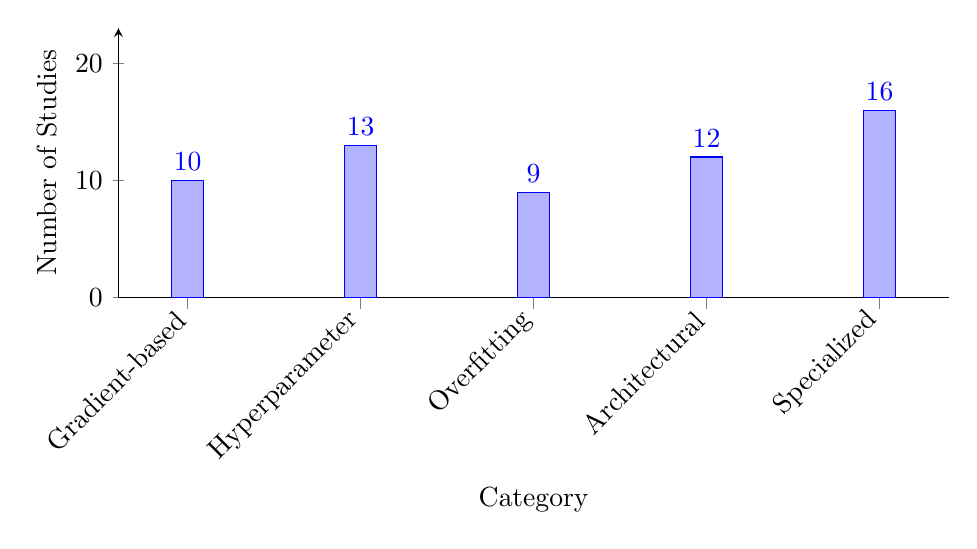
\begin{tikzpicture}
\begin{axis}[
    ybar,
    bar width=0.4cm,
    % enlargelimits=0.5,
     enlarge x limits=.1,
    ylabel={Number of Studies},
    xlabel={Category},
    symbolic x coords= {
        Gradient-based, Hyperparameter, Overfitting, Architectural, Specialized
    },
    xticklabel style={rotate=45, anchor=east},
    xtick=data,
    nodes near coords,
    ymin=0,
    ymax=23,
    axis x line*=bottom,
    axis y line=left,
    width=\textwidth,
    height=5cm
]
\addplot coordinates {
    (Gradient-based,10)
    (Hyperparameter,13)
    (Overfitting,9)
    (Architectural,12)
    (Specialized,16)
};
\end{axis}
\end{tikzpicture}
\caption{Number of reviewed studies utilizing each category of optimization technique.}
\label{fig:optimization-distribution}
\end{figure}

\renewcommand{\arraystretch}{1.35}
\begin{table*}[t]
\centering
\caption{Summary of Optimization Techniques in Deep Learning for Oncology}
\label{tab:optimization-techniques}
\begin{tabular}{|p{4cm}|p{4cm}|p{4cm}|}
\hline
\textbf{Category} & \textbf{Description} & \textbf{Examples} \\
\hline
Gradient-based optimizers & Update network weights via gradient descent algorithms & SGD, NAG, Adam, Adagrad, SAdagrad \\
\hline
Hyperparameter tuning & Search for optimal settings like learning rate, number of layers & Grid Search, Random Search, PSO, Bayesian Optimization \\
\hline
Overfitting reduction & Improve generalization by reducing overfitting risk & Dropout, Batch Normalization, L1/L2 Regularization, Early Stopping \\
\hline
Data strategies & Enhance training through data preprocessing and augmentation & Transfer Learning, Data Augmentation, PCA, SMOTE, Autoencoders \\
\hline
Architectural enhancements & Modify model structure or use biologically inspired design & P-NET, BioNet, CNN-GA, Multi-task Learning, Evolutionary Design \\
\hline
Specialized methods & Support privacy, explainability, or complex decision processes & Federated Learning (FL), DRL \\
\hline
\end{tabular}
\end{table*}



\subsection{Author's method}
W celu uzupełnienia przeglądu literatury przeprowadzono niezależny eksperyment, mający na celu ocenę wpływu wybranych technik optymalizacji na wydajność głębokiej sieci konwolucyjnej (CNN) w zadaniu klasyfikacji obrazów raka piersi. Wykorzystano publicznie dostępny zbiór danych BreakHis, który stanowi standardowy punkt odniesienia w badaniach histopatologicznych. Zbiór ten zawiera 9 109 mikroskopowych obrazów tkanki guza piersi, pobranych od 82 pacjentek przy użyciu mikroskopu optycznego w czterech różnych powiększeniach: 40×, 100×, 200× oraz 400×. Każdy obraz, zapisany w formacie RGB o rozdzielczości 700 × 460 pikseli, jest oznaczony jako łagodny lub złośliwy i przypisany do jednego z ośmiu podtypów. Należy podkreślić, że zbiór jest niezbalansowany, z przewagą próbek złośliwych.
Jako model bazowy przyjęto prostą sieć CNN składającą się z trzech warstw konwolucyjnych, trenowaną przy użyciu stochastycznego spadku gradientu (SGD) z domyślnym współczynnikiem uczenia 0,01. Następnie wprowadzano różnorodne techniki optymalizacji i modyfikacje architektoniczne, aby zmierzyć ich wpływ względem bazy. Wydajność oceniano za pomocą standardowych metryk: dokładności, precyzji, czułości (recall), wyniku F1 oraz AUC, a także monitorowano czas treningu i walidacji w celu oceny efektywności obliczeniowej. Wszystkie eksperymenty zaimplementowano w środowisku PyTorch na systemie Windows 10, zachowując spójność potoku przetwarzania wstępnego. Celem analizy jest określenie, jak poszczególne strategie wpływają na wyniki klasyfikacji oraz zużycie zasobów w rzeczywistych warunkach.

\section{Experimental Evaluation}
Celem ewaluacji eksperymentalnej była szczegółowa ocena wpływu pojedynczych oraz łączonych technik optymalizacji na wydajność i efektywność obliczeniową głębokich sieci neuronowych w zadaniu klasyfikacji obrazów raka piersi. Badanie porównawcze przeprowadzono na autorskim modelu CNN trenowanym na zbiorze BreakHis, analizując zarówno metryki predykcyjne, jak i czasy wykonania. Aby zapewnić rzetelność wyników, każda konfiguracja modelu była testowana w ramach 5-krotnej stratyfikowanej walidacji krzyżowej, z ograniczeniem do trzech epok treningowych na każdy fold. Punktem odniesienia (baseline) była konfiguracja wykorzystująca optymalizator stochastycznego spadku gradientu (SGD) bez żadnych dodatkowych ulepszeń regularyzacyjnych czy preprocesingu.
Następnie testowano szereg modyfikacji przypisanych do sześciu głównych kategorii optymalizacji w onkologii zdefiniowanych wcześniej w artykule. W ramach optymalizatorów gradientowych porównano SGD z algorytmami Adagrad i Adam. Dostrajanie hiperparametrów objęło testy różnych wartości współczynnika uczenia (learning rate). W celu redukcji przeuczenia zastosowano warstwy Dropout oraz normalizację wsadową (Batch Normalization). Strategie danych uwzględniały standardową augmentację obrazów oraz Transfer Learning z wykorzystaniem sieci DenseNet-121 (jako ekstraktora cech oraz w trybie fine-tuning). Ulepszenia architektoniczne polegały na dodaniu czwartej warstwy konwolucyjnej do autorskiego CNN oraz na całkowitym zastąpieniu go architekturą DenseNet-121. Wydajność oceniano za pomocą metryk: dokładność, precyzja, czułość (recall), F1-score oraz AUC, a także poprzez pomiar czasu treningu i walidacji, co pozwoliło na identyfikację kompromisów między jakością predykcji a kosztami obliczeniowymi.


\subsection{Setup}


% \begin{figure}
% \centering
% \begin{tikzpicture}[
%     layer/.style={rectangle, draw=black, fill=blue!10, minimum width=2.5cm, minimum height=1cm, font=\small},
%     conv/.style={rectangle, draw=black, fill=orange!20, minimum width=3.5cm, minimum height=1cm, font=\small},
%     dense/.style={rectangle, draw=black, fill=green!20, minimum width=3.5cm, minimum height=1cm, font=\small},
%     output/.style={rectangle, draw=black, fill=red!20, minimum width=3.5cm, minimum height=1cm, font=\small}
% ]

% \node[layer] (input) {Input: $3 \times 128 \times 128$};
% \node[conv, below=0.8cm of input] (conv1) {Conv1: $16@128\times128$};
% \node[conv, below=0.6cm of conv1] (conv2) {Conv2: $32@64\times64$};
% \node[conv, below=0.6cm of conv2] (conv3) {Conv3: $64@32\times32$};
% \node[layer, below=0.6cm of conv3] (flatten) {Flatten: $64 \times 16 \times 16$};
% \node[dense, below=0.6cm of flatten] (fc1) {FC1: 128 + ReLU};
% \node[output, below=0.6cm of fc1] (fc2) {FC2: 2 classes (Softmax)};

% \draw[->] (input) -- (conv1);
% \draw[->] (conv1) -- (conv2);
% \draw[->] (conv2) -- (conv3);
% \draw[->] (conv3) -- (flatten);
% \draw[->] (flatten) -- (fc1);
% \draw[->] (fc1) -- (fc2);

% \end{tikzpicture}
% \caption{Architecture of the custom CNN model used in the experiment.}
% \label{fig:cnn-architecture}
% \end{figure}


Eksperymenty zaimplementowano w języku Python z użyciem biblioteki PyTorch na systemie Windows 10 wyposażonym w procesor graficzny NVIDIA. Podstawą badania był zbiór BreakHis, zawierający 9 109 obrazów histopatologicznych o rozdzielczości 700×460 pikseli, obejmujących cztery poziomy powiększenia (40×–400×). Obrazy te, podzielone na klasy łagodne i złośliwe, zostały poddane 5-krotnej stratyfikowanej walidacji krzyżowej, co zapewniło reprezentatywność klas w każdym przebiegu testowym.
Autorska architektura CNN, zaprojektowana jako lekki model bazowy, składa się z trzech warstw konwolucyjnych (z filtrami o rozmiarach odpowiednio 16, 32 i 64, funkcją aktywacji ReLU i poolingiem), po których następuje spłaszczenie mapy cech i dwie warstwy w pełni połączone (FC). Dane wejściowe przeskalowano do formatu 128×128 RGB. W wariancie rozszerzonym dodano czwarty blok konwolucyjny ze 128 filtrami, aby zwiększyć pojemność modelu. Proces treningowy wykorzystywał funkcję straty entropii krzyżowej (cross-entropy loss) oraz optymalizator SGD z domyślnym learning rate 0,01, momentum 0,9 i brakiem wygaszania wag. Rozmiar wsadu (batch size) ustalono na 32, a trening trwał przez 3 epoki bez użycia early stoppingu. Dla każdej konfiguracji rejestrowano szereg metryk wydajności oraz czas obliczeń, co umożliwiło kompleksową analizę błędów i efektywności.

\subsection{Observations and Analysis}

Analiza wyników eksperymentalnych przedstawionych w Tabeli \ref{tab:results-summary} i \ref{tab:time-accuracy-summary} ujawnia wyraźne trendy dotyczące skuteczności poszczególnych strategii optymalizacyjnych. Spośród optymalizatorów gradientowych, Adagrad zdecydowanie przewyższył bazowy SGD oraz algorytm Adam, osiągając dokładność 88,03\% oraz imponujący wskaźnik AUC równy 0,95. Wynik ten uzyskano przy minimalnym wzroście czasu treningu, co potwierdza skuteczność adaptacyjnego doboru tempa uczenia. Zaskakująco słabo wypadł popularny optymalizator Adam, uzyskując najniższą dokładność w tej grupie (71,48\%), co może sugerować jego niestabilność w specyficznych warunkach tego eksperymentu.
Ręczne strojenie hiperparametrów okazało się nieskuteczne – modyfikacje współczynnika uczenia (0,001 i 0,0001) dały gorsze rezultaty niż ustawienia domyślne, co podkreśla wyższość metod adaptacyjnych. W zakresie redukcji przeuczenia, Batch Normalization okazał się jednym z najlepszych podejść niearchitektonicznych, podnosząc dokładność do 85,72\% i AUC do 0,94, podczas gdy Dropout zapewnił solidną stabilizację wyników. Z kolei proste techniki, takie jak augmentacja danych czy dodanie czwartej warstwy konwolucyjnej, nie przyniosły oczekiwanych korzyści (odpowiednio 81,90\% i 82,00\%), co może wynikać z wysokiej zmienności samego zbioru BreakHis lub ryzyka przeuczenia przy głębszej strukturze.
Bezapelacyjnym zwycięzcą okazał się Transfer Learning z wykorzystaniem sieci DenseNet-121. Tryb Fine-Tuning pozwolił na osiągnięcie niemal perfekcyjnej dokładności 99,72\% oraz AUC 0,9988, deklasując pozostałe metody. Jest to jednak okupione najwyższym kosztem obliczeniowym – warianty DenseNet wymagały około 6800 sekund całkowitego czasu wykonania, w porównaniu do około 5800–6000 sekund dla modeli opartych na autorskim CNN. Podsumowując, eksperymenty dowiodły, że strategie oparte na dynamice treningu i zaawansowanych architekturach wstępnie wytrenowanych są znacznie bardziej efektywne niż naiwne modyfikacje strukturalne czy ręczne strojenie parametrów.



% \begin{table}[h]
% \centering
% \caption{Performance Summary by Optimization Category (5-Fold Cross-Validation)}
% \label{tab:results-summary}
% \begin{tabular}{|l|l|c|c|c|c|c|}
% \hline
% \textbf{Optimization Category} & \textbf{CNN Configuration} & \textbf{Accuracy [\%]} & \textbf{Macro F1} & \textbf{AUC} & \textbf{Precision} & \textbf{Recall} \\ \hline
% \multirow{3}{*}{Gradient-based Optimizer} 
%     & \makecell[l]{CNN (3-layer)\\ baseline}           & 84.36 $\pm$ 0.61 & 0.81 & 0.85 & 0.83 & 0.79 \\ \cline{2-7}
%     & \cellcolor{lightgreen}Adagrad         & \cellcolor{lightgreen}\textbf{88.03} $\pm$ 1.07 & \cellcolor{lightgreen}\textbf{0.86} & \cellcolor{lightgreen}\textbf{0.95} & \cellcolor{lightgreen}\textbf{0.87} & \cellcolor{lightgreen}\textbf{0.85} \\ \cline{2-7}
%     & \makecell[l]{Adam}             & 71.48 $\pm$ 5.67 & 0.48 & 0.57 & 0.44 & 0.55 \\ \hline

% \multirow{2}{*}{Hyperparameter Tuning} 
%     & \makecell[l]{Learning Rate\\ = 0.0001}       & 68.64 $\pm$ 0.00 & 0.41 & 0.62 & 0.34 & 0.50 \\ \cline{2-7}
%     & \makecell[l]{Learning Rate\\ = 0.001}        & 73.90 $\pm$ 6.49 & 0.55 & 0.83 & 0.71 & 0.59 \\ \hline

% \multirow{2}{*}{Overfitting Reduction} 
%     & Dropout                     & 84.26 $\pm$ 0.92 & 0.80 & 0.85 & 0.84 & 0.78 \\ \cline{2-7}
%     & Batch Normalization         & 85.72 $\pm$ 8.77 & 0.78 & 0.94 & 0.90 & 0.79 \\ \hline

% Data Strategy 
%     & Data Augmentation           & 81.90 $\pm$ 4.72 & 0.75 & 0.84 & 0.83 & 0.74 \\ \hline

% \makecell[l]{Architectural \\ Enhancement} 
%     & \makecell[l]{Added 4th\\ Conv Layer}         & 82.00 $\pm$ 2.22 & 0.77 & 0.84 & 0.83 & 0.76 \\ \hline

% \multirow{3}{*}{\makecell[l]{Transfer Learning /\\ Fine-Tuning}}  
%     & \makecell[l]{DenseNet121}     & 85.76 $\pm$ 0.55 & 0.90 & 0.92 & 0.86 & 0.94 \\ \cline{2-7}
%     & \cellcolor{lightblue}DenseNet121 + Fine-Tuning & \cellcolor{lightblue}\textbf{99.72} $\pm$ 0.09 & \cellcolor{lightblue}\textbf{0.9980} & \cellcolor{lightblue}\textbf{0.9988} & \cellcolor{lightblue}\textbf{0.9972} & \cellcolor{lightblue}\textbf{0.9999} \\ \cline{2-7}
%     & \makecell[l]{DenseNet121 +\\ Transfer Learning} & 89.48 $\pm$ 1.75 & 0.92 & 0.97 & 0.93 & 0.92 \\ \hline

% \end{tabular}
% \end{table}


% \begin{table*}[h]
% \centering
% \caption{Accuracy and Execution Time Summary by Optimization Category}
% \label{tab:time-accuracy-summary}
% \begin{tabular}{|l|l|c|c|c|}
% \hline
% \textbf{Optimization Category} & 
% \textbf{CNN Configuration} & 
% \makecell{\textbf{Accuracy} \\ \textbf{[\%]}} &
% \makecell{\textbf{Avg. Training} \\ \textbf{Time / Fold} \\ {[s]}} & 
% \makecell{\textbf{Total Execution} \\ \textbf{Time} \\ {[s]}} \\

% \hline

% \multirow{3}{*}{Gradient-based Optimizer} 
%     & \makecell[l]{CNN (3-layer) baseline} & 84.36 $\pm$ 0.61 & 1072.90 & 5799.46 \\ \cline{2-5}
%     & \cellcolor{lightgreen}Adagrad & \cellcolor{lightgreen}\textbf{88.03} $\pm$ 1.07 & \cellcolor{lightgreen}1094.80 & \cellcolor{lightgreen}5884.82 \\ \cline{2-5}
%     & Adam & 71.48 $\pm$ 5.67 & 1106.30 & 5944.94 \\ \hline

% \multirow{2}{*}{Hyperparameter Tuning} 
%     & \makecell[l]{Learning Rate = 0.0001} & 68.64 $\pm$ 0.00 & 1107.15 & 5955.52 \\ \cline{2-5}
%     & \makecell[l]{Learning Rate = 0.001} & 73.90 $\pm$ 6.49 & 1113.09 & 5988.21 \\ \hline

% \multirow{2}{*}{Overfitting Reduction} 
%     & Dropout & 84.26 $\pm$ 0.92 & 1100.95 & 5923.42 \\ \cline{2-5}
%     & Batch Normalization & 85.72 $\pm$ 8.77 & 1141.17 & 6131.82 \\ \hline

% Data Strategy 
%     & Data Augmentation & 81.90 $\pm$ 4.72 & 1147.88 & 6154.77 \\ \hline

% Architectural Enhancement 
%     & \makecell[l]{Added 4th Conv Layer} & 82.00 $\pm$ 2.22 & 1108.47 & 5978.06 \\ \hline

% \multirow{3}{*}{\makecell[l]{Transfer Learning /\\ Fine-Tuning}} 
%     & \makecell[l]{DenseNet121 (frozen)} & 85.76 $\pm$ 0.55 & 1354.03 & 6770.13 \\ \cline{2-5}
%     & \cellcolor{lightblue}DenseNet121 + Fine-Tuning & \cellcolor{lightblue}\textbf{99.72} $\pm$ 0.09 & \cellcolor{lightblue}\textbf{1364.10} & \cellcolor{lightblue}\textbf{6820.49} \\ \cline{2-5}
%     & \makecell[l]{DenseNet121 + Transfer Learning} & 89.48 $\pm$ 1.75 & 1341.44 & 6707.20 \\ \hline

% \end{tabular}
% \end{table*}

\subsection{Comparision with Literature Results}
Porównanie uzyskanych wyników z literaturą przedmiotu dostarcza istotnego kontekstu. Jak pokazano wcześniej w Tabeli 1, zoptymalizowane modele DL w onkologii często osiągają skuteczność w przedziale 95–99\%, a rekordowe rozwiązania, takie jak AMCNN czy LFR-COA-DenseNet121, notują wyniki rzędu 99,7\%–99,97\%. Nasz najlepszy wynik – 99,72\% uzyskany dzięki dostrajaniu (fine-tuning) sieci DenseNet-121 – jest w pełni zbieżny z tymi rezultatami, co potwierdza potencjał zaawansowanych architektur.
Jednakże nasze prostsze modele trenowane od podstaw osiągnęły znacznie niższe wyniki (np. 88,03\% dla CNN z Adagradem, a zaledwie 71,48\% dla Adama). Rozbieżności te wynikają z czterech kluczowych czynników. Po pierwsze, literatura opiera się zazwyczaj na głębokich architekturach (ResNet, hybrydy z atencją), które lepiej ekstrahują złożone cechy niż nasz lekki CNN. Po drugie, czas treningu w naszym eksperymencie ograniczono rygorystycznie do 3 epok, podczas gdy badania literaturowe stosują setki epok, co pozwala na pełniejszą konwergencję. Po trzecie, brak zaawansowanego preprocessingu (normalizacja barw, segmentacja ROI) w naszym podejściu utrudnił modelowi naukę na zróżnicowanych danych BreakHis. Wreszcie, złożoność zadania – klasyfikacja podtypów w BreakHis jest trudniejsza niż proste problemy binarne często opisywane w innych pracach.

\subsection{Interpretation and Practical Implications}

Wyniki te niosą konkretne implikacje praktyczne. Adaptacyjne optymalizatory, takie jak Adagrad, oferują znaczną poprawę wyników względem SGD przy znikomym wzroście kosztów obliczeniowych, co czyni je idealnym wyborem dla środowisk o ograniczonych zasobach sprzętowych. Z kolei w krytycznych systemach diagnostycznych, gdzie priorytetem jest maksymalna precyzja, najlepszym rozwiązaniem pozostaje fine-tuning głębokich sieci (np. DenseNet-121), mimo wyższych wymagań obliczeniowych. Warto również podkreślić rolę Batch Normalization jako skutecznego stabilizatora dla płytszych sieci.
Badanie to posiada jednak ograniczenia: krótki czas treningu (3 epoki) mógł nie pozwolić na pełne wykorzystanie potencjału niektórych metod, a brak zaawansowanych technik wyjaśnialności (XAI) ogranicza zaufanie kliniczne. Ponadto, brak augmentacji w wariantach transfer learningu oraz ograniczona wielkość próby w BreakHis mogły wpłynąć na generalizację.



\subsection{Future Work}
Przyszłe prace powinny koncentrować się na wydłużeniu procesu treningowego z zastosowaniem mechanizmu early stopping, co pozwoli na lepszą konwergencję modeli. Obiecującym kierunkiem jest wdrożenie zaawansowanych harmonogramów uczenia oraz algorytmów metaheurystycznych (np. SWChOA), a także łączenie technik, które wykazały skuteczność w izolacji (np. Adagrad z Batch Normalization). Kluczowe dla wdrożeń klinicznych będzie zintegrowanie narzędzi wyjaśnialności (Grad-CAM, SHAP) oraz testowanie innych architektur (ResNet, EfficientNet) w kontekście treningu uwzględniającego specyfikę powiększeń obrazów mikroskopowych.

